\documentclass[10pts, letterpaper]{article}
\usepackage[]{float}
\usepackage[utf8]{inputenc}
\usepackage[T1]{fontenc}
\usepackage{textcomp}
\usepackage[dutch]{babel}
\usepackage{amsmath, amssymb}
\usepackage[margin=1.3in]{geometry}
\usepackage{import}
\usepackage{xifthen}
\pdfminorversion=7
\usepackage{pdfpages}
\usepackage{transparent}
\newcommand{\incfig}[1]{%
	\def\svgwidth{\columnwidth}
	\import{./figures/}{#1.pdf_tex}
}
\usepackage[]{fancyhdr}
\pdfsuppresswarningpagegroup=1

\setlength\parindent{0pt}
\begin{document}
\pagestyle{fancy}
\fancyhead{} % clear all header fields
\fancyhead[L]{PHYS301 : Classical Mechanics}
\fancyhead[C]{\rightmark}
\fancyhead[R]{Homework 05}
\fancyfoot{}
\renewcommand{\footrulewidth}{0.4pt}

\newlength\adder
\setlength\adder{1cm}
\addtolength\headwidth{2\adder}
\fancyheadoffset{\adder}

\fancyfoot[C]{\vspace{0.3cm}\\ \thepage}

\allowdisplaybreaks

\begin{center}
\ 
	\vspace{1cm} 

	\Huge{\textsf{Homework 06 : : Classical Mechanics}}
	\\
	\vspace{1cm}
	\Large{\texttt{Ahmed Saad Sabit}}
	\vspace{1.5cm} 
\end{center}
{\flushright
\section*{Answer Sheet} 
}
\newpage
\ 


\section*{Problem 01} 
\subsection*{(a)}

Because the question states the sentence ``for times $t$ after the driving force has ceased'' - I am going to assume the following function for the force
\[
F_\text{ext} (t) =
\begin{cases}
	mA \sin(\omega_1 t) & 0 < t < N \frac{2 \pi }{\omega_1} 
	\\
	0 & t \ge N \frac{2 \pi }{\omega_1}
\end{cases}
\quad 
\text{where} \quad \omega_1 ^2 = \omega_0^2 - \beta^2
\]
for the given equation of motion 
\[
\ddot{x} + 2 \gamma \dot{x} + \omega_0^2 = F_\text{ext}(t)
\] 

For Green's method to find the oscillator response
\begin{align*}
	\frac{\mathrm{d} ^2G(t,t')}{\mathrm{d} t^2 	 }
	+ 
2 \gamma	\frac{\mathrm{d} G(t,t')}{\mathrm{d} t} 
+ 
\omega_0^2 G(t,t') &= \delta(t - t')\\
\left(
\frac{\mathrm{d} ^2}{\mathrm{d} t^2} + 2 \gamma \frac{\mathrm{d} }{\mathrm{d} t} + \omega_0
^2\right) G(t, t') f(t') &=  \delta(t - t') f(t') \\ 
\left(
\frac{\mathrm{d} ^2}{\mathrm{d} t^2} + 2 \gamma \frac{\mathrm{d} }{\mathrm{d} t} + \omega_0
^2 \right) 
\int_{-\infty}^{\infty} \mathrm{d} t' G(t, t') f(t') &= \int_{-\infty}^{\infty} \mathrm{d} t' f(t') = f(t) =   
\left(
\frac{\mathrm{d} ^2}{\mathrm{d} t^2} + 2 \gamma \frac{\mathrm{d} }{\mathrm{d} t} + \omega_0
^2 \right)  x(t) \\
\implies 
\int_{-\infty}^{\infty} f(t') G(t, t') \, \mathrm{d} t' &= 
x(t)
\end{align*}
The required integral 
\begin{align*} x(t) &=   
	\int_{-\infty}^{\infty} f(t') G(t,t') \mathrm{d} t' \\ & = 
	\int_{-\infty}^{0} f(t') G(t,t') \mathrm{d} t' + 
	\int_{0}^{N \frac{2\pi }{\omega_1}} f(t') G(t,t') \mathrm{d} t' + 
	\int_{N \frac{2 \pi }{\omega_1}}^{\infty} f(t') G(t,t') \mathrm{d} t'  \\ 
	&=  0 + \int_{0}^{N \frac{2\pi }{\omega_1}} f(t') G(t,t') \mathrm{d} t' +  0 \\
	&= \int_{0}^{N \frac{2  \pi }{\omega_1 }}   mA \sin( \omega_1 t' ) G(t,t') \mathrm{d} t' \\
	&= 
\int_{0}^{N \frac{2 \pi }{\omega_1}}  
m A \sin ( \omega_1 t') 
\left(
\Theta(t - t') e^{ - \gamma (t - t' ) } 
\frac{1}{\omega_1 } \sin 
\left(
\omega_1 (t - t' )
\right)
\right)\, \mathrm{d} t' 
	\\
	&= 
\int_{0}^{N \frac{2 \pi }{\omega_1}}  
m A \sin ( \omega_1 t') 
\left(
\Theta(t - t') e^{- \gamma t} e^{\gamma t ' }
\frac{1}{\omega_1 } 
\left[
\sin(\omega_1 t) \cos(\omega_1 t' ) - 
\cos(\omega_1 t) \sin(\omega_1 t') 
\right]
\right)\, \mathrm{d} t' 
	\\
	&= \frac{m A}{\omega_1}  
\int_{0}^{N \frac{2 \pi }{\omega_1}}  
\left(
 \Theta(t - t') e^{- \gamma (t - t' ) } \sin(\omega_1 t' )
\left[
\sin(\omega_1 t) \cos(\omega_1 t' ) - 
\cos(\omega_1 t) \sin(\omega_1 t') 
\right]
\right)\, \mathrm{d} t' 
	\\ 
 &= \frac{m A}{\omega_1}  
\left[
 \int_{t}^{N \frac{2 \pi }{\omega_1}}   \mathrm{d} t'\, 
e^{ - \gamma (t - t ') }
\sin(\omega_1 t) \sin(\omega_1 t') \cos(\omega_1 t' ) - 
\int_{t}^{N \frac{2 \pi }{\omega_1}}   \mathrm{d} t' \,
e^{ - \gamma  (t - t ') }
\cos(\omega_1 t) \sin^2(\omega_1 t') 
\right] \tag{note lower bound of integration has changed to $t$} 
\end{align*}
Please note that $\omega_1 > \gamma$ here by definition.  
\begin{align*}
	\int_{t}^{N \frac{2 \pi }{\omega}} \mathrm{d} x \, e^{- \gamma ( t- x) } \sin(\omega t) \sin(\omega x) \cos(\omega x) &=  - 
\sin( \omega t) 
\frac{
\left(
{\gamma} ^2
\sin\left(2t{\omega}\right) 
- 
2 {\omega} \gamma 
\cos\left(2t{\omega}\right) + 
2{\omega}\gamma \mathrm{e}^{\gamma \left(
\frac{2 N \pi{}}{\omega}  - t\right)} \right)}
{8\gamma{\omega}^{2} + 2 {\gamma}^{3}} 
\\
	\int_{t}^{N \frac{2 \pi }{\omega_1}}   \mathrm{d} x\, 
e^{ -\gamma (t-x)} \sin(\omega_1 t) \sin^2 (\omega_1 x) &=  
\sin\left({\omega} t\right) \left(\frac{2{\gamma}{\omega} \sin\left(2t{\omega}\right) + {\gamma}^{2} \cos\left(2t{\omega}\right) - 4{\omega}^{2} - {\gamma}^{2}}{8{\gamma}{\omega}^{2} + 2{\gamma}^{3}} + 
\frac{ 4 {\omega}^{2} 
\mathrm{e}^{\gamma\left(\frac{2N\pi{}}{\omega} - t \right)}}{{8{\gamma}}{ {\omega}^{2} + 2 {\gamma}^{3} } } \right)
\end{align*}


Wait. 
\\
What the hell am I doing. 
\\
I could have just integrated $\sin (\omega_1 (t - t')) $ directly on a integral calculator.
\\
I am such an idiot. 
\\
Let me do this all over again. Starting from 
\begin{align*}
	\int_{0}^{N \frac{2\pi}{\omega_1}}  m A \sin(\omega_1 t') G(t, t') \, \mathrm{d} t' 
	&= 
\frac{mA}{\omega_1} 
\int_{0}^{N \frac{2\pi}{\omega_1}}   \mathrm{d} t' \, 
\Theta(t-t') e^{ - \gamma (t - t') } 
\sin(\omega_1 t') 
\sin(\omega_1 (t - t'))
	\\ 
	&= 
\frac{mA}{\omega_1} 
\int_{t}^{N \frac{2\pi}{\omega_1}} \mathrm{d} t' 
\, 
e^{- \gamma (t-t' ) } 
\sin(\omega_1 t' ) \sin(\omega_1 (t - t')) 
	\\
	&= 
\frac{mA}{\omega_1} 
\left(
- \frac{\omega_1}{\gamma} 
\frac{
\gamma  \sin(\omega_1 t)
\left[ 
	\exp\left(\gamma ( \frac{2 N \pi }{\omega_1 } - t) \right) + 1
\right]
+
2 \omega  \cos(\omega_1 t)
\left[ 
	\exp\left(\gamma ( \frac{2 N \pi }{\omega_1 } - t) \right) - 1 
\right]
}{4 \omega_1^2 + \gamma^2} 
\right)
	\\
	x(t) &= 
 - m A 
\left(
\frac{
\sin(\omega_1 t)
\left[ 
	\exp\left(\gamma ( \frac{2 N \pi }{\omega_1 } - t) \right) + 1
\right]
+
( 2 \omega / \gamma )  \cos(\omega_1 t)
\left[ 
	\exp\left(\gamma ( \frac{2 N \pi }{\omega_1 } - t) \right) - 1 
\right]
}{4 \omega_1^2 + \gamma^2} 
\right)
	\\
\end{align*}
The integral calculator gave me 
\[
	\int_{t}^{10 \pi / \omega_1}  \mathrm{d} x \,  
	\sin\left({\omega} \left(t - x\right)\right) \, \mathrm{e}^{-{\gamma} \left(t - x\right)} \sin\left({\omega}x\right)= 
-\frac{\mathrm{e}^{-t{\gamma}} {\omega} \left(\left({\gamma}\mathrm{e}^{\frac{10\pi{\gamma}}{\omega}} + {\gamma}\mathrm{e}^{t{\gamma}}\right) \sin\left(t{\omega}\right) + \left(2{\omega}\mathrm{e}^{\frac{10\pi{\gamma}}{\omega}} - 2\mathrm{e}^{t{\gamma}} {\omega}\right) \cos\left(t{\omega}\right)\right)}{{\gamma} \left(4{\omega}^{2} + {\gamma}^{2}\right)}
\] 
where $N = 5$. If you want $\beta$ definition then substitute $2 \gamma = \beta$ for proper $\beta$ form. We did $2 \gamma$ in class so I went with that.

\subsection*{b}
We know for $x \to  0$ without $x = 0$, 
\[
e^{x} \approx 1 + x
\] 
For ridiculously small $\gamma$, 
Then 
\[
\exp \left(
\gamma 
\left(\frac{2 N \pi }{\omega_1 } - t\right)
\right) \pm 1  
=
\gamma 
\left(\frac{2 N \pi }{\omega_1 } - t\right) + 1 \pm 1 
\]
And of course  
\[
2 \frac{\omega}{\gamma} \gg 1 
\]
So we are left with 
 \[
 x(t) \approx - \frac{mA}{4 \omega_1^2} 
 \left( \frac{2 \omega }{ \gamma }\right)
\gamma 
\left(\frac{2 N \pi }{\omega_1 } - t\right)
 \cos(\omega_1 t) =
 \frac{mA}{2 \omega_1} 
\left( t- \frac{2 N \pi }{\omega_1 } \right)
 \cos(\omega_1 t)
 \] 
 There is a linear increase the amplitude starting from a negative. By the time $t = \frac{2 N \pi }{\omega_1}$ there is no oscillation. But then as $t$ grows the oscillation amplitude begins to increase. Hence in case of negligible $\gamma$, the phase of force is such that it kills the original oscillation and starts to grow again. 
\section*{Problem 02} 


\subsection*{Polar Coordinates} 
The radius, azimuth and inclination (angle wrt. to $\hat{z}$) being $r, \theta, \phi$ 
\begin{align*}
	x &= r \cos \theta \sin \phi \\
	y &= r \sin \theta \sin \phi \\
	z &= r \cos \phi
\end{align*}
Polar and Cartesian coordinate transformation in differential form
\begin{align*}
	p_i \to (p_1,p_2, p_3 ) &= (r, \theta, \phi) \\
	x_i \to (x_1,x_2,x_3) &= (x,y,z) \\ 
	\vec{e}_{p_i} = 
	\frac{\partial \vec{R}}{\partial p_i} &= \sum_{j= 1}^{3}
\frac{\partial \vec{R}}{\partial x_j} \frac{\mathrm{d} x_j}{\mathrm{d} p_i}
	\\
\end{align*} Hence for instance we get 
\[
\vec{e}_r = \frac{\partial \vec{R}}{\partial r} = 
\frac{\partial \vec{R}}{\partial x} 
\frac{\mathrm{d} x}{\mathrm{d} r} + 
\frac{\partial \vec{R}}{\partial y} 
\frac{\mathrm{d} y}{\mathrm{d} r} + 
\frac{\partial \vec{R}}{\partial z} 
\frac{\mathrm{d} z}{\mathrm{d} r}
\]
Noting that 
\[
\frac{\partial \vec{R}}{\partial x} = \vec{e}_x 
\] 
We can write
\[
\vec{e}_r = \frac{\partial \vec{R}}{\partial r} = 
\cos \theta \sin \phi \vec{e}_x + 
\sin \theta \sin \phi \vec{e}_y + 
\cos \phi \vec{e}_z 
\]
For all coordinates, 
\begin{align*}
	\vec{e}_r &= 
\cos \theta \sin \phi \vec{e}_x + 
\sin \theta \sin \phi \vec{e}_y + 
\cos \phi \vec{e}_z 
\\ 
\vec{e}_\theta &= 
-r \sin \theta \sin \phi \vec{e}_x + 
r \cos \theta \sin \phi \vec{e}_y 
\\
\vec{e}_\phi &= 
r \cos \theta \cos \phi \vec{e}_x + 
r \sin \theta \cos \phi \vec{e}_y - 
r \sin \phi \vec{e}_z \\
\end{align*}
We require the derivative of this set of unit vectors now to get velocity. One way could be computationally grind the derivatives, and the other way could be defining the angular velocity $\vec{\omega}$ and then taking a cross product. [Idea bought from Asian Physics Olympiad 2019 T3 Tippe Top Problem] 

Rotation purely so that $| \vec{\omega} | = \dot{\theta}$ results in rotation purely about $\hat{z} = \vec{e}_z$ axis. 

Rotation pure so that $|  \vec{\omega} | = \dot{\phi}$ results in rotation purely about $\vec{e}_\theta$ axis [please consult the diagram]

\begin{figure}[H]
	\centering
	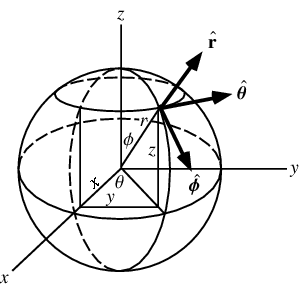
\includegraphics[width=0.5\textwidth]{ss/6/coord.png}
	\caption{Diagram of notations}
	\label{fig:}
\end{figure}

\begin{align*}
	\vec{\omega} &= \dot{\phi} \vec{e}_\theta + \dot{\theta} \vec{e}_z	 \\
&= \dot\theta \cos\phi \vec{e}_r + \dot \phi \vec{e}_\theta - \dot \theta \sin \phi \vec{e}_\phi \\
\end{align*}
	      \begin{align*}
              \dot{\vec{e}}_r &= \vec{\omega} \times \vec{e}_r
              = \dot\theta \cos\phi \, \vec{e}_r \times \vec{e}_r
              + \dot\phi \, \vec{e}_\theta \times \vec{e}_r
              - \dot\theta \sin\phi \, \vec{e}_{\phi} \times \vec{e}_r \\
              \dot{\vec{e}}_{\theta} &= \vec{\omega} \times \vec{e}_{\theta}
              = \dot\theta \cos\phi \,\vec{e}_r \times \vec{e}_\theta
              + \dot\phi \, \vec{e}_\theta \times \vec{e}_\theta
              - \dot\theta \sin\phi \,\vec{e}_{\phi} \times \vec{e}_\theta \\
              \dot{\vec{e}}_{\phi} &= \vec{\omega} \times \vec{e}_{\phi}
              = \dot\theta \cos\phi \,\vec{e}_r \times \vec{e}_\phi
              + \dot\phi \, \vec{e}_\theta \times \vec{e}_\phi
              - \dot\theta \sin\phi \,\vec{e}_{\phi} \times \vec{e}_\phi
              \end{align*}

	  \begin{align*}
              \dot{\vec{e}}_r &= \dot\theta \sin\phi \,\vec{e}_{\theta}
              + \dot\phi \,\vec{e}_{\phi} \\
              \dot{\vec{e}}_{\theta} &= - \dot\theta \sin\phi \,\vec{e}_r
              - \dot\theta \cos\phi \,\vec{e}_{\phi} \\
              \dot{\vec{e}}_{\phi} &= - \dot\phi \,\vec{e}_r
              + \dot\theta \cos\phi \,\vec{e}_{\theta}
              \end{align*}

	     Now we are ready to take acceleration in polar basis because we know individual derivatives in terms of $p_i$ 's. Setting $\vec{R} = \vec{R}(r, \theta, \phi)$
	     \begin{align*}
		     \vec{R} &= R \vec{e}_r \\
		     \vec{v} = \frac{\mathrm{d} \vec{R}}{\mathrm{d} t} &= 
		     \dot{R} \vec{e}_r + R \dot{\vec{e}}_r = \dot{R} \dot{\vec{e}}_r + 
		     R \dot{\theta} \sin \phi \vec{e}_\theta + R \dot{\phi} \vec{e}_\phi
	     \end{align*}
	     \begin{align*}
              \vec{a} = \dot{\vec{v}} &= \frac{\mathrm{d} }{\mathrm{d} t}\Big(
              \dot{R} \,\vec{e}_r
              + R \dot\theta \sin\phi \,\vec{e}_{\theta}
              + R \dot\phi \,\vec{e}_{\phi} \Big) \\
              &= \ddot{R} \, \vec{e}_r + \dot{r} \, \dot{\vec{e}}_r
              + (\dot{R} \dot\theta \sin\phi + r \ddot\theta \sin\phi
              + R \dot\theta \cos\phi \, \dot\phi) \, \vec{e}_\theta \\
              &\quad + R \dot\theta \sin\phi \, \dot{\vec{e}}_\theta
              + (\dot{R} \dot\phi + r \ddot\phi) \, \vec{e}_\phi
              + r \dot\phi \, \dot{\vec{e}}_\phi \\ 
\vec{a} &= (\ddot{R} - R \dot{\theta}^2 \sin^2\phi
              - R \dot{\phi}^2) \,\vec{e}_r \\
              &\quad + (R \ddot\theta \sin\phi
              + 2 \dot{R} \dot\theta \sin\phi
              + 2 R \dot\theta \dot\phi \cos\phi) \,\vec{e}_{\theta} \\
              &\quad + (R \ddot\phi + 2 \dot{R} \dot\phi
              - r \dot{\theta}^2 \sin\phi \cos\phi) \,\vec{e}_{\phi}
              \end{align*}

	      \subsection*{Cylinderical Coordinates} 
	      Now unfortunately I don't have the will power or energy to ninja techniq the last result to turn that into Cylinderical coordinates. I know there's some basic algebraic manipulation I could do but I don't want to think so hard I am tired. 

	      I will do this from scratch, again. It's more work but no thinking. 

	      I am gonna use the same angular velocity technique to avoid taking the painful derivative. 

	      \begin{align*}
	      	x &=  r \cos \theta \\
		y &= r \sin \theta \\
		z &= z \\
	      \end{align*}
	     Now for a general vector in cylinderical representation 
	     \[
	     \vec{\rho} = r \cos \theta \vec{e}_x + r \sin \theta \vec{e}_y + z \vec{e}_z
	     \] 
The transform 
	     \begin{align*}
              \vec{e}_r &= \frac{\partial\vec{\rho}}{\partial r}
              = \cos\theta \, \vec{e}_x
              + \sin\theta \, \vec{e}_y \\
              \vec{e}_\theta &= \frac{\partial\vec{\rho}}{\partial\theta}
              = -r \sin\theta \, \vec{e}_x
              + r \cos\theta \, \vec{e}_y \\
              \vec{e}_z &= \frac{\partial\vec{\rho}}{\partial z}
              = \vec{e}_z
              \end{align*}
	      The rotation 
	      \[
	      \vec{\omega} = \dot \theta \vec{e}_z
	      \]
The derivative computation 
	      \begin{align*}
              \dot{\vec{e}}_r &= \vec{\omega} \times \vec{e}_r
              = \dot\theta \, \vec{e}_z \times \vec{e}_r
              = \dot{\theta} \, \vec{e}_\theta \\
              \dot{\vec{e}}_{\theta} &= \vec{\omega} \times \vec{e}_{\theta}
              = \dot\theta \, \vec{e}_z \times \vec{e}_\theta
              = - \dot\theta \, \vec{e}_r \\
              \dot{\vec{e}}_z &= \vec{\omega} \times \vec{e}_{\phi}
              = \dot\theta \, \vec{e}_z \times \vec{e}_z
              = 0
              \end{align*}
The derivative
	      \begin{align*}
              \dot{\vec{e}}_r &= \dot\theta \, \vec{e}_{\theta} \\
              \dot{\vec{e}}_{\theta} &= - \dot\theta \, \vec{e}_r \\
              \dot{\vec{e}}_z &= 0
              \end{align*}
	Now one by one, 
	\begin{align*}
		\vec{\rho} &= r \vec{e}_r + z \vec{e}_z \\	
		\vec{v} = \dot{\vec{\rho}} &= \dot{r} \vec{e}_r + r \dot\vec{e}_r + \dot{z} \vec{e}_z + z \dot \vec{e}_z\\
		&= \dot{r} \vec{e}_r + r \dot \theta \vec{e}_\theta + \dot{z} \vec{e}_z \\
		\vec{a} = \ddot{\vec{\rho}}&=  
\ddot{r} \vec{e}_r + 
\dot{r} \dot{\vec{e}}_r + 
(\dot r \dot \theta + r \ddot{\theta} ) \vec{e}_\theta + 
r \dot \theta \vec{e}_\theta + \ddot{z} \vec{e}_z + \dot{z} \dot{\vec{e}}_z 
		\\
		&= 
		(\ddot{r} - r \dot{\theta}^2) \vec{e}_r + 
		(r \ddot{\theta} + 2 \dot{r} \dot{\theta} ) \vec{e}_\theta + 
		\ddot{z} \vec{e}_z
		\\
	\end{align*}
\section*{Problem 03} 
Inspired by the action quantity 
\[
	J = \int \, \mathcal{L }[q, \dot{q}, t] \, \mathrm{d} t
\] 
\begin{align*}
	J &= \int \, \sqrt{\mathrm{d} t^2 + \gamma \mathrm{d} s ^2 }\\ 
	&=  \int \mathrm{d} s \sqrt{ 
		\left(\frac{\mathrm{d} t}{\mathrm{d} s}\right)^2 + \gamma
	} \\
	&= 
\int \mathrm{d} x
\sqrt{1 + \left( \frac{\mathrm{d} y}{\mathrm{d} x}\right)^2 } 
\sqrt{ \left(\frac{\mathrm{d} t}{\mathrm{d} s}\right)^2 + \gamma } 
	\\
	&= 
\int
\mathrm{d} x \, 
\sqrt{1 + y'(x) ^2 } 
\sqrt{\frac{1}{v(x)^2} + \gamma} \\
	&= 
\int
\mathrm{d} x \, 
\sqrt{1 + y' (x )^2 } 
\sqrt{\frac{1}{2 g x } + \gamma} 
\end{align*}

The equivalent EL-equations 
\[
\frac{\mathrm{d} }{\mathrm{d} x} 
\frac{\partial \mathcal L }{\partial y'}  = 
\frac{\partial \mathcal L}{\partial y} = 
\frac{\partial \mathcal L[y'(x), x] }{\partial y} =  0 
\]
\begin{align*}
	\frac{\partial \mathcal L }{\partial y'} &= 
\frac{y'(x)}{\sqrt{1 + y'(x)^2 }  } 
\sqrt{\frac{1}{2 g x} + \gamma } 
	\\
	\frac{\mathrm{d} }{\mathrm{d} x } \frac{\partial \mathcal L }{\partial y'} &= 
\frac{\mathrm{d} }{\mathrm{d} x} \left( y'(x) \frac{1}{\sqrt{1 + y'(x)^2 }  } 
\sqrt{\frac{1}{2 g x} + \gamma } 
\right) 	= 0 \\
										   &\implies
 y'(x) \frac{1}{\sqrt{1 + y'(x)^2 }  } 
 \sqrt{\frac{1}{2 g x} + \gamma }  = C  \tag{$C$ is dummy constant} \\ 
										   &\implies
										   y'(x)^2
										   \frac{1}{1 + y'(x)^2}
										   \left(
\frac{1}{2g x}  + \gamma 
										   \right) = C
\end{align*}
\begin{align*}
&\implies
y'(x) ^2 \frac{1}{1 + y'(x)^2} = \frac{C}{\frac{1}{2gx} + \gamma} \\
&\implies
\frac{1 + y'(x)^2 }{y'(x)^2} -1 = \frac{ \frac{1}{2gx} + \gamma }{C} - 1 \\ 
&\implies
y'(x) = \sqrt{\frac{C}{ \frac{1}{2gx} + \gamma - C}} 
\end{align*}
To solve this 
\begin{align*}
	\frac{\mathrm{d} y}{\mathrm{d} x} &= \sqrt{\frac{C}{ \frac{1}{2gx } + \gamma - C}}  \\
	y &= \int \, \mathrm{d} x 
	\sqrt{\frac{C}{ \frac{1}{2gx } + \gamma - C}}  
\end{align*}

\subsection*{General $\gamma$ solution} 
\begin{figure}[H]
	\centering
	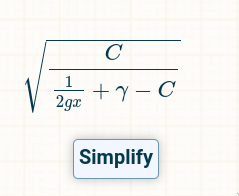
\includegraphics[width=0.4\textwidth]{ss/6/integral.png}
	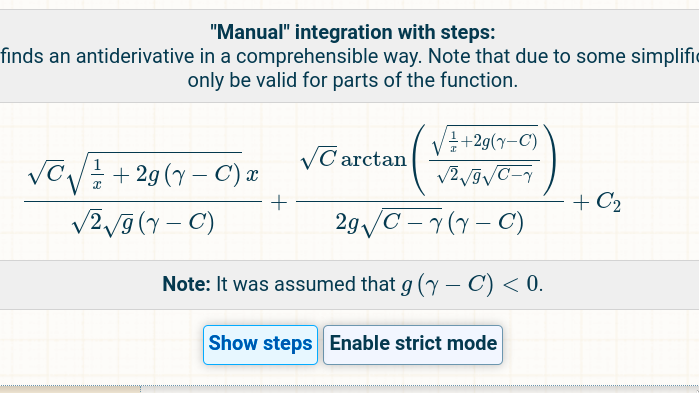
\includegraphics[width=0.4\textwidth]{ss/6/solution.png}
	\caption{ss/6/solution.png}
	\label{fig:ss-6-solution-png}
\end{figure}
\[ y(x) = 
\frac{\sqrt{C} \sqrt{\frac{1}{x} + 2g \left({\gamma} - C\right)} \, x}{\sqrt{2} \sqrt{g} \left({\gamma} - C\right)} + \frac{\sqrt{C} \arctan\left(\frac{\sqrt{\frac{1}{x} + 2g \left({\gamma} - C\right)}}{\sqrt{2} \sqrt{g} \sqrt{C - {\gamma}}}\right)}{2g \sqrt{C - {\gamma}} \left({\gamma} - C\right)}
\] 
\subsection*{$\gamma = 0$} 
This minimizes $\int \mathrm{d} t$ so we should expect a cartesian cycloid solution. 
Taking the original differential equation we got, 
\begin{align*}
	\left(
\frac{1}{2g x} + \gamma - C
	\right) y'(x)^2 &=  C \\ 
	\frac{1 + y'^2}{y'^2}  &= \frac{\gamma}{C} + \frac{1}{2 Cg x } \\ 
	\frac{\mathrm{d} x}{\mathrm{d} y}^2 \left(
	1 + \frac{\mathrm{d} y}{\mathrm{d} x}^2\right) &= \frac{\gamma}{C} + \frac{1}{2 C g x} \\ 
	\implies 
	x'^2 + 1 &= \frac{\gamma}{C} + \frac{1}{2 g C x}  \\
	\implies 
	(x'^2 + 1) 2gC x &= 1 \\
	\implies
	\text{cycloid} \\
	x &= gc(1 - \cos \theta) \\
	y &= gc(\theta - \sin \theta) \\
\end{align*}

\subsection*{$\gamma \gg 1$ } 
When $\gamma \gg 1$ then we have 
\begin{align*}
	y &= \int \mathrm{d} x \, 
\sqrt{\frac{C}{\gamma }}  
	\\
	\implies 
	y &= M x + D \\
\end{align*}
Where $y = y(x)$ is a straight line. This makes sense because then we have $J = \int \gamma \, \mathrm{d} s$ where path is optimized. 




\newpage 
\section*{TRASHCAN: room for aesthetic latex i cannot erase because i typed them with blood and tears} 
\begin{align*}
	&= 
	\frac{m A}{\omega_1 }e^{ - \gamma t} 
	\left[
\omega_1 \frac{1 - e^{ \gamma \frac{2 \pi N }{ \omega_1 } } }{4 \omega_1 ^2 + \psi ^2 } \sin (\omega_1 t) - 
\frac{2 \omega_1^2 }{\gamma } \frac{e^{\gamma \frac{2 \pi N }{\omega_1 } } - 1 }{4 \omega_1 ^2 + \gamma^2 } \sin(\omega_1 t )
	\right]
	\\
	&= 
	\frac{m A}{\omega_1 }e^{ - \gamma t} 
	\left[
\omega_1 \frac{1 - e^{ \gamma \frac{2 \pi N }{ \omega_1 } } }{4 \omega_1 ^2 + \gamma ^2 } \sin (\omega_1 t) +
\frac{2 \omega_1^2 }{\gamma } \frac{1-e^{\gamma \frac{2 \pi N }{\omega_1 } } }{4 \omega_1 ^2 + \gamma^2 } \sin(\omega_1 t )
	\right]
     \\ &=
	\frac{mA}{\omega_1} e^{- \gamma t} 
	\left(\frac{1 - e^{ \gamma \frac{2 \pi N}{\omega_1 } } }{4 \omega_1 ^2 + \gamma^2 }
		\right) \sin(\omega_1 t)
		\left[ \omega_1 - \frac{2 \omega_1^2 }{\gamma} \right]
     \\ &=
	mA
	\left(\frac{1 - e^{ \gamma \frac{2 \pi N}{\omega_1 } } }{4 \omega_1 ^2 + \gamma^2 }
		\right) 
		\left[ 1 - \frac{2 \omega_1 }{\gamma} \right] e^{- \gamma t} \sin(\omega_1 t)
     \\ &=
	mA
	\left(\frac{ e^{ \gamma \frac{2 \pi N}{\omega_1 } } - 1 }{4 \omega_1 ^2 + \gamma^2 }
		\right) 
		\left[  \frac{2 \omega_1 }{\gamma} - 1 \right] e^{- \gamma t} \sin(\omega_1 t)
     \\ &=
	mA
	\left(\frac{ e^{ \gamma \frac{2 \pi N}{\omega_1 } } - 1 }{4 \omega_1 ^2 + \gamma^2 }
		\right) 
		\left[  \frac{2 \omega_1 }{\gamma} - 1 \right] e^{- \gamma t} \sin(\omega_1 t) 
		\tag{$\omega_1 = \sqrt{\omega_0^2 - \gamma^2} $}
\end{align*}
\end{document}
